\documentclass[11pt]{article}

\usepackage[T1]{fontenc}
\usepackage[utf8]{inputenc}
\usepackage{charter}
\usepackage[scaled=0.9]{helvet}
\usepackage{courier}
\usepackage[margin=1in]{geometry}
\usepackage{microtype}
\usepackage{amsmath,amssymb}
\usepackage{booktabs}
\usepackage{tabularx}
\usepackage{longtable}
\usepackage{array}
\usepackage{enumitem}
\usepackage[dvipsnames]{xcolor}
\usepackage{tikz}
\usetikzlibrary{arrows.meta,positioning,calc,shapes.geometric,fit}
\usepackage{fancyvrb}
\usepackage[hidelinks]{hyperref}
\usepackage{titlesec}
\usepackage{caption}

\setlist{itemsep=2pt,topsep=4pt}
\setlength{\parskip}{4pt}
\setlength{\parindent}{0pt}
\setlength{\emergencystretch}{2.5em}
\renewcommand{\arraystretch}{1.18}
\captionsetup{font=small,labelfont=bf}

\usepackage{url}
\urlstyle{tt}
\makeatletter
\g@addto@macro{\UrlBreaks}{\do\_\do\:\do\-\do\,}
\makeatother
\newcommand{\code}{\path}
\newcolumntype{L}{>{\raggedright\arraybackslash}X}
\newcolumntype{P}[1]{>{\raggedright\arraybackslash}p{#1}}

\definecolor{accent}{RGB}{176,58,46}
\definecolor{soft}{RGB}{245,240,236}
\definecolor{ok}{RGB}{39,110,72}

\newenvironment{keypoint}{\begin{center}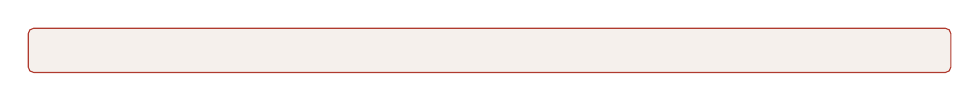
\begin{tikzpicture}\node[draw=accent,fill=soft,rounded corners=2pt,inner sep=8pt,text width=0.92\linewidth]\bgroup}{\egroup;\end{tikzpicture}\end{center}}

\title{\textbf{Breaking the Validator Stall Loop}\\[4pt]
\large Cost-accounted order-then-execute for F1R3Node:\\ analysis, design, and development plan}
\author{F1R3FLY.io --- design document, revision 2}
\date{October 16, 2026}

\begin{document}
\maketitle

\begin{center}
\small
\begin{tabular}{@{}lP{10.6cm}@{}}
\toprule
Repository & \code{F1R3FLY-io/f1r3node-rust} \\
Stall review basis & \code{master} at \code{7264c98} (Oct 15, 2026) \\
Branch reviewed & \code{feature/cost-accounted-rho} at \code{ccbee928} (Oct 13, 2026) \\
Integration target & \code{dev} at \code{555a5e44} (Oct 16, 2026) \\
Revision 2 & Incorporates the Casper Working Group response to \S5.10.1 and the status of delivered work (Oct 16, 2026) \\
Method & Code reading with line-level verification. No profiling was run for this document. \\
\bottomrule
\end{tabular}
\end{center}

\begin{abstract}
\noindent Validators stall as they come under sustained load. A code review traces the stall to a set of feedback loops that all feed on one quantity: the finality lag, the distance between the tips of the block DAG and the last finalized block (LFB). Many per-block and per-proposal costs grow with that lag, which slows proposals and validation, which lengthens the lag. Two hard limits then turn the slowdown into a stop. The root of most of this cost is run-to-completion execution: because each deploy runs to completion against a committed state, concurrently produced blocks hold divergent post-states, and the node must merge them. The cost-accounting design removes the reason for the merge. Every potential conflict is marked by signature, so deploys can run at any time, and agreement reduces to two things: the state changes of each block, settled by one runner and checked by replay, and the order of conflicting blocks. This document reports the stall analysis, assesses how much of it the \code{feature/cost-accounted-rho} branch addresses today, gives a detailed design for cost-accounted order-then-execute on v6 shards, and lays out a development plan that lands it in \code{dev} with minimal change to the legacy path. Revision~2 replaces the finalizer-progress rule of revision~1, which was unsafe, with a design that separates a resumable computation, a validation under the commit-time snapshot, and an atomic commit (\S\ref{sec:finalizer}). It also records the work delivered so far.
\end{abstract}

\tableofcontents
\newpage

%======================================================================
\section{Summary}

\textbf{The problem.} Under sustained deploy load, the unfinalized region of the DAG grows. Proposal preparation, merging, the deploy lifecycle register and the finality oracle all do work that grows with that region. Their combined cost delays blocks and finality, which grows the region further. Two limits close the trap: the finalizer discards any run that takes longer than 15 seconds, and merges refuse outright once the floor distance exceeds 256 blocks. Separately, consensus CPU work runs on the same asynchronous worker threads as networking, so a busy node also stops answering its peers. Section~\ref{sec:analysis} gives the evidence.

\textbf{The cause underneath.} In \code{dev}, each deploy runs to completion; the only concurrency is the parallel composition inside a deploy. A block's post-state is therefore a function of one linear sequence of deploys. Two concurrent blocks start from a common pre-state and end in divergent post-states, so something must reconcile them. That reconciliation is the merge, and the merge is the largest consumer of the costs that grow with the lag.

\textbf{The resolution.} Under cost accounting, every potential conflict is marked by signature, including races on shared data channels between different signers. Deploys can then run at any time and interleave freely. All conflict resolution moves to the block level, where validators need to agree only on (i) the state changes of each block, which decide the winners of every race, and (ii) the order of conflicting blocks. The first is settled by one runner and verified by replay; the second, in a first version, by a total order on finalized blocks. No sequential scheduler is involved.

\textbf{The branch today.} \code{feature/cost-accounted-rho} implements the cost-accounting core and a funding gate, but its Casper pipeline is still execute-then-merge. Its interim v6 merge rule removes the exponential conflict search on v6 shards. Otherwise the stall loop is untouched, a v6 block carries at most one user deploy, and the reducer changes cost legacy shards 15--23\,\% more CPU on the branch's own profiles. The branch's own design proposal (its \S7) describes order-then-execute but keeps deploy-at-a-time execution and a single-order scheduler. This document corrects both.

\textbf{Finality progress.} Revision~1 said that a finalizer run that reaches its deadline ``adopts the highest candidate proven so far''. The Casper Working Group showed that this rule is not safe and gives no progress argument (\S\ref{sec:finalizer}). An oracle verdict on one candidate is not a finality decision. Revision~2 adopts the group's replacement: a resumable \emph{Compute} phase, a \emph{Validate} phase under the snapshot at commit time, and an atomic \emph{Commit}. A deadline never cancels Validate or Commit, and no partial result is ever committed. The delivered fix A1a was already consistent with this. It keeps only facts about immutable blocks across runs and commits only complete derivations.

\textbf{The plan.} Two tracks run in parallel (Section~\ref{sec:plan}). Track~A fixes the stall on \code{dev} now, independent of cost accounting, and those fixes are prerequisites for v6 as well, because the finality half of the loop survives any execution model. Track~B lands cost accounting in \code{dev} in seven increments. The legacy path stays byte-identical to \code{dev}. The interim merge rule, the one-offer block lane and the scheduler are left behind. The v6 consensus seam enters through four hook points behind a genesis-policy switch. Track~A is delivered, with A9 off by default, as is the first v6 tranche (\S\ref{sec:status}).

\begin{keypoint}
\textbf{Decisions recorded for this design (October 16, 2026).}
\begin{enumerate}[label=(\arabic*),leftmargin=1.5em]
\item The single-order reduction scheduler is superseded by an order-independent charge model. The scheduler-based decision records are superseded or amended accordingly (\S\ref{sec:charge}).
\item Signature marking covers data-channel races between different signers. Two blocks conflict only if their signature footprints intersect (\S\ref{sec:footprint}).
\item A first version uses a total order on finalized blocks; exploiting the partial order is a later refinement.
\item The finalizer adopts a candidate only after a complete derivation and a re-validation under the commit-time snapshot. The commit is one atomic transaction. This supersedes \S5.10.1 of revision~1 (\S\ref{sec:finalizer}).
\end{enumerate}
\end{keypoint}

%======================================================================
\section{The stall: analysis}\label{sec:analysis}

\subsection{The core loop}

Under sustained load three quantities grow together: the pending deploy pool, the set of deploys included in blocks but not yet settled, and the unfinalized DAG cone. Each grows with the finality lag $D$ (tip height minus LFB height), and each carries costs that scale with it (Figure~\ref{fig:loop}).

\begin{figure}[h]
\centering
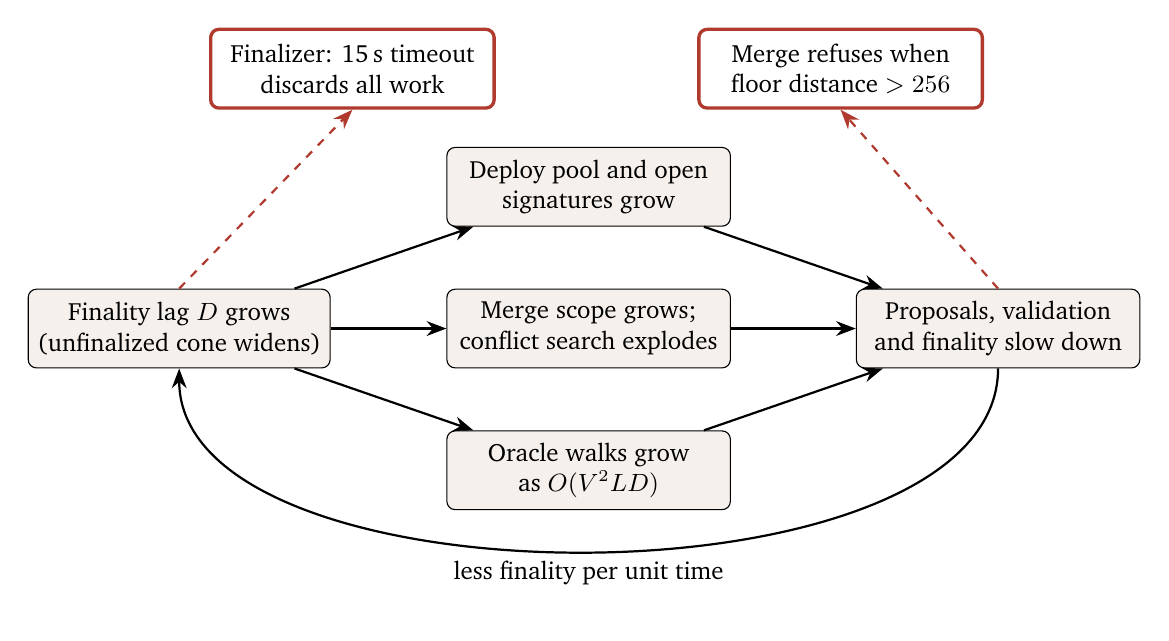
\begin{tikzpicture}[
  box/.style={draw,rounded corners=3pt,fill=soft,align=center,minimum width=3.6cm,minimum height=1.0cm,font=\small},
  trap/.style={draw=accent,very thick,rounded corners=3pt,fill=white,align=center,minimum width=3.6cm,minimum height=1.0cm,font=\small},
  arr/.style={-{Stealth[length=2.5mm]},thick}]
\node[box] (lag) at (0,0) {Finality lag $D$ grows\\(unfinalized cone widens)};
\node[box] (pool) at (5.2,1.8) {Deploy pool and open\\signatures grow};
\node[box] (merge) at (5.2,0) {Merge scope grows;\\conflict search explodes};
\node[box] (fin) at (5.2,-1.8) {Oracle walks grow\\as $O(V^2 L D)$};
\node[box] (slow) at (10.4,0) {Proposals, validation\\and finality slow down};
\draw[arr] (lag) -- (pool);
\draw[arr] (lag) -- (merge);
\draw[arr] (lag) -- (fin);
\draw[arr] (pool) -- (slow);
\draw[arr] (merge) -- (slow);
\draw[arr] (fin) -- (slow);
\draw[arr] (slow.south) .. controls (10.4,-3.6) and (0,-3.6) .. node[below,font=\small]{less finality per unit time} (lag.south);
\node[trap] (t1) at (2.2,3.3) {Finalizer: 15\,s timeout\\discards all work};
\node[trap] (t2) at (8.4,3.3) {Merge refuses when\\floor distance $>256$};
\draw[arr,accent,dashed] (lag.north) -- (t1.south);
\draw[arr,accent,dashed] (slow.north) -- (t2.south);
\end{tikzpicture}
\caption{The feedback loop. Every cost on the middle column grows with the finality lag; the two traps (outlined) turn the slowdown into a stop.}
\label{fig:loop}
\end{figure}

Two limits turn the slowdown into a stall:
\begin{enumerate}
\item \textbf{The finalizer timeout.} \code{finalization_runner.rs:278-293} wraps each finalizer run in a 15-second \code{tokio::time::timeout}. On timeout the run is dropped and nothing is adopted. Each later run starts from scratch over a larger cone, so once one run exceeds 15\,s the LFB never advances again. A non-zero \code{finalizer.run.timeouts} counter marks entry into this regime.
\item \textbf{The floor-distance cap.} \code{interpreter_util.rs:956} sets \code{MAX_FLOOR_DISTANCE_BLOCKS = 256}. Beyond it, \code{compute_parents_post_state} refuses: proposers park and validators reject. If every validator crosses the cap, the shard can deadlock, because advancing finality may itself need new blocks.
\end{enumerate}

\subsection{Costs that grow with the lag}

Each item below was verified at the cited lines. Complexity is stated in the quantity that grows under load.

\begin{longtable}{@{}P{3.6cm}P{6.3cm}P{5.4cm}@{}}
\toprule
\textbf{Mechanism} & \textbf{Where and what} & \textbf{Growth} \\
\midrule
\endhead
Deploy pool re-read under a lock &
\code{block_creator.rs:590} takes the pool's \code{parking_lot::Mutex} and holds it to about line 1495. Proposal preparation reaches \code{read_all()} about four times over the pool and the rejected buffer. Decoding goes through \code{Signed::from_signed_data} (\code{casper_message.rs:1363}), which re-verifies every signature. &
About $8N$ signature checks per proposal, $N$ the pool size. $N$ grows with lag because included-but-unsettled deploys stay in the pool by design (\code{block_admission.rs:169}). No admission cap. \\
Lineage walks per deploy &
\code{effect_in_state_of} (\code{deploy_lifecycle.rs:93-155}) calls \code{block_store.get}, which decodes and verifies every deploy of each block, once per selected deploy, per buffered deploy, and per open signature on each floor advance. &
Open signatures $\times$ segment length $\times$ deploys per block: quadratic in load. \\
Rejection-option search &
\code{compute_rejection_options} (\code{merging_logic.rs:1270-1407}): breadth-first over keep/reject choices, cloning the conflict map per option; duplicate check is a linear scan (\code{:1369}). Components sharing any mergeable channel are unioned (\code{conflict_set_merger.rs:905-917}), and the search is re-run until a fixed point (\code{dag_merger.rs:705-752}). &
Exponential in conflicting pairs per group; vault and PoS channels collapse groups into one. Runs on both proposal and validation. \\
Hot channels in RSpace &
Data values are plain \code{Vec<Datum>} in \code{imbl} shards (\code{hot_store.rs:402}): deep-copied on first write after each soft checkpoint, cloned on read, shifted by \code{insert(0, ..)}, and re-serialized at checkpoint. Replay clones per candidate and walks candidates in $O(K^2)$ (\code{replay_rspace.rs:799, 950, 1117-1145}). &
$O(n)$ per touch, $O(n^2)$ over a run for a channel accumulating $n$ datums. \\
Finality walks &
Every lookup is an LMDB read plus a full metadata decode; \code{is_dag_ancestor} is a fresh BFS, called $O(P^2)$--$O(P^3)$ times per floor derivation; the clique oracle makes a new run cache per call (\code{clique_oracle.rs:793}). &
$O(P \cdot V^2 L D)$ warm, $O(D^2)$ cold, per block. \\
Full table scans under the DAG lock &
\code{get_representation_internal} calls \code{to_map()} on latest messages and invalid blocks (\code{block_dag_key_value_storage.rs:1199-1207}); invalid blocks are never deleted. A read-only equivocation scan takes the global \emph{write} lock (\code{:1570}) twice per block. &
Grows with history; serializes readers including the proposer's snapshot. \\
\bottomrule
\end{longtable}

\subsection{Bottlenecks and starvation}

\begin{itemize}
\item \textbf{Proposer queue.} With auto-propose on, every deploy spawns its own propose request with up to four retries (\code{block_api.rs:499-515}) into a 1{,}024-entry queue drained serially, 250\,ms plus a full proposal per entry. The ``already in progress'' branch is unreachable, because the consumer awaits the proposal inline (\code{proposer_instance.rs:181}). Deploy-triggered requests run in the heartbeat lane, so they can mint empty blocks that every peer must replay.
\item \textbf{Synchronous locks in async code.} Concurrent \code{do_deploy} calls park worker threads on the pool mutex while a proposal holds it. When waiting deploys equal the worker count, the runtime, including transport, stops.
\item \textbf{CPU work on the async runtime.} Replay, \code{dag_merger::merge}, checkpoints and block creation run on tokio workers without \code{spawn_blocking}; two parallel validations plus a proposal can pin 3--4 workers and starve gRPC, peer-to-peer traffic and the heartbeat.
\item \textbf{Heartbeat and polling.} Every accepted block and deploy wakes the heartbeat, whose snapshot cache misses on every insert. gRPC \code{find_deploy} retries up to $80 \times 100$\,ms per request, scanning 128 heights per miss.
\end{itemize}

\subsection{Two defects independent of load}

\begin{itemize}
\item \textbf{Buffer eviction removes the newest block.} \code{casper_buffer_key_value_storage.rs:335-341} computes age as \code{now - first_seen}, sorts ascending, and removes the first entry, which is the youngest pendant, often the block that just became ready. It also re-sorts the whole buffer per removal.
\item \textbf{Re-fetch defeats its own rate limit.} \code{recover_stale_buffer_dependencies} re-requests parents already in the buffer from four peers; the duplicate reply is dropped as \code{AlreadyProcessed}, and that path clears both the cooldown and the retry counter.
\end{itemize}

\subsection{Soak evidence}

The branch's own proposal (\code{docs/casper/theory/cost-accounting-consensus-proposal.md}, \S9.1) records two soaks. In the August soak one merge call averaged 2.16\,s, of which the settled-signature probes took 92\,\%, and the probe depth grew with the finality lag; \code{dev} has since batched those probes. In the October soak no single stage separated failing sessions from passing ones (AUC at most 0.70), and \code{dev}'s analysis points to the finality round length and to blocks waiting for missing parents. Read together with the code review, the binding constraint has moved from merge analysis toward finality and Casper bookkeeping. Any design must therefore fix finality as well as remove the merge.

%======================================================================
\section{Why the merge exists, and how cost accounting removes it}\label{sec:why}

\subsection{Run-to-completion}

In \code{dev}, RSpace accepts a deploy, runs it to termination or until its phlogiston is exhausted, commits the state, and only then accepts the next deploy. The only concurrency inside a block is the parallel composition within a deploy. A block's post-state is a function of the parent state and one sequence of deploys.

Validators propose concurrently. Two blocks built on a common ancestor each run their own sequences and end in different post-states. A child with both as parents must combine them: decide which deploys conflict, choose which to reject, and compose the rest. That is the merge, with its event-log indexes, its conflict maps and its rejection-option search. Every block must also be replayed by every validator before acceptance, because its post-state is part of its validity. Merge and replay are the two consensus-path costs that grow with the unfinalized cone.

\subsection{Conflicts marked by signature}

The cost-accounting papers replace run-to-completion with concurrent acceptance gated by linear resource proofs. Every interaction draws tokens from the signatures involved:
\begin{itemize}
\item deploys with \emph{different} signatures draw from disjoint pools and cannot conflict on funding;
\item deploys with the \emph{same} signature compete for one pool and are serialized by the linear proof;
\item races on shared data channels between different signers are also marked by signature: every communication is charged to each participant's signature, so two deploys that race for the same datum or continuation both draw on the signature that owns the contested process (decision~2).
\end{itemize}
The branch's linear cost estimate already counts every participant of a communication: a receive with $n$ binds has $n+1$ participants (proposal \S4.1). The runtime must charge them the same way; \S\ref{sec:footprint} gives the test. With every potential conflict marked by signature, conflicts become visible at the level of signatures rather than discovered after the fact from event logs.

\subsection{Agreement reduces to two things}

Deploys can then run at any time and interleave. Nothing requires a block's effect to equal some sequential order of its deploys. Validators need to agree on exactly two things:
\begin{enumerate}
\item \textbf{The state changes of each block}, which decide, for the whole shard, the winner of every race in it. One runner executes the block and records the outcome; every other node replays the record to verify it.
\item \textbf{The order of conflicting blocks.} Blocks whose signature footprints are disjoint commute. A first version simply totally orders all finalized blocks; a refinement orders only conflicting ones.
\end{enumerate}
A sequential scheduler is \emph{not} needed for agreement and is harmful to throughput: it manufactures determinism by discarding concurrency, when agreement only needs the race winners, which a record already carries.

\begin{figure}[h]
\centering
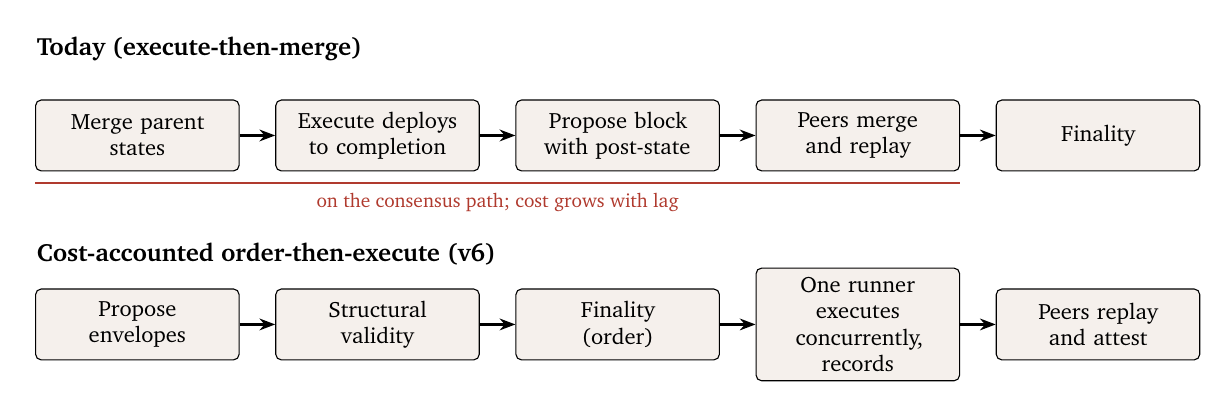
\begin{tikzpicture}[
  st/.style={draw,rounded corners=2pt,fill=soft,align=center,font=\footnotesize,minimum height=0.9cm,text width=2.35cm},
  arr/.style={-{Stealth[length=2mm]},thick}]
\node[font=\small\bfseries,anchor=west] at (-1.4,1.1) {Today (execute-then-merge)};
\node[st] (a1) at (0,0) {Merge parent\\states};
\node[st] (a2) at (3.05,0) {Execute deploys\\to completion};
\node[st] (a3) at (6.1,0) {Propose block\\with post-state};
\node[st] (a4) at (9.15,0) {Peers merge\\and replay};
\node[st] (a5) at (12.2,0) {Finality};
\foreach \x/\y in {a1/a2,a2/a3,a3/a4,a4/a5} \draw[arr] (\x) -- (\y);
\node[font=\small\bfseries,anchor=west] at (-1.4,-1.5) {Cost-accounted order-then-execute (v6)};
\node[st] (b1) at (0,-2.4) {Propose\\envelopes};
\node[st] (b2) at (3.05,-2.4) {Structural\\validity};
\node[st] (b3) at (6.1,-2.4) {Finality\\(order)};
\node[st] (b4) at (9.15,-2.4) {One runner executes\\concurrently, records};
\node[st] (b5) at (12.2,-2.4) {Peers replay\\and attest};
\foreach \x/\y in {b1/b2,b2/b3,b3/b4,b4/b5} \draw[arr] (\x) -- (\y);
\draw[accent,thick] ($(a1.south west)+(0,-0.15)$) -- ($(a4.south east)+(0,-0.15)$) node[midway,below,font=\scriptsize,text=accent]{on the consensus path; cost grows with lag};
\end{tikzpicture}
\caption{Moving execution behind ordering. In the lower pipeline, consensus never merges or replays.}
\label{fig:pipelines}
\end{figure}

%======================================================================
\section{The branch as it stands}\label{sec:branch}

\code{feature/cost-accounted-rho} is 501 commits ahead of its merge base with \code{dev} (\code{93e38575}, Oct 6) and 470 behind, about 507{,}000 added lines. Of those, 184{,}000 are formal proofs and models, 63{,}000 design documents, 113{,}000 the Rholang interpreter (94{,}000 in \code{accounting/}), 29{,}000 RSpace, 18{,}000 models, and 39{,}000 Casper (35{,}000 in the new \code{costacc/} module). A trial merge into today's \code{dev} conflicts in 38 files.

\subsection{Effect on the loop}

\begin{longtable}{@{}P{5.2cm}P{9.8cm}@{}}
\toprule
\textbf{Loop component} & \textbf{Effect of the branch} \\
\midrule
\endhead
Finalizer timeout, floor-distance cap & Not touched (\code{floor.rs} $+3/-3$). \\
Pool re-reads under lock & Not touched; v6 adds offered-envelope scans under the same lock. \\
Lineage walks, lifecycle register & Not touched. \\
Rejection-option search & Replaced on v6 shards only by one ordered pass (\code{dag_merger.rs:1862-1882}, DR-120). The merge index, the larger cost (8--10\,\% of test work against 1--1.6\,\% for the merge call), remains. \\
Hot-channel copies & Priced, not removed: the native replay store charges for copies, and v6 host-work caps bound them. Representation unchanged. \\
Finality walks, proposer queue, heartbeat, runtime starvation & Not touched. \\
\bottomrule
\end{longtable}

Two further effects work against throughput:
\begin{itemize}
\item \textbf{One user deploy per v6 block.} Once a first offered candidate is chosen, every later one becomes a fallback (\code{block_creator.rs}, about line 1910). Multi-offer blocks (G2-2 onward) are approved but not started. Under load, the pool, and therefore the lag, grows faster on v6 than on legacy.
\item \textbf{Legacy shards pay for the reducer changes.} The scheduler (\code{deterministic_reduction.rs}) and the accounting sit inside \code{ReducerCore} for every shard. The branch's profiles show 15--23\,\% more CPU than \code{dev} on legacy multi-parent tests, outside the merge.
\end{itemize}

\subsection{The branch's own order-then-execute proposal}

The branch carries a proposal (\S7 of the document named above) for order-then-execute on v6 shards. It gets the architecture right in three respects: a canonical total order of finalized blocks along the main chain; one runner with verified replay (since the October 13 amendment); and structural block validity with no merge, execution or replay on the consensus path. It departs from the model of Section~\ref{sec:why} in two respects that this design corrects:
\begin{enumerate}
\item \textbf{Its executor is deploy-at-a-time.} Proposal \S7.6 holds, executes and settles one envelope before the next, and \S7.10 admits a parallel executor only if its result replays as that sequential batch. That re-imports run-to-completion into the executor.
\item \textbf{It keeps the single-order scheduler, or serial replay.} Under native execution every RSpace operation of a deploy joins one conflict component (\code{deterministic_reduction.rs:1068-1072, 1120-1122}) and runs alone. The scheduler exists because some host-work charges read live container sizes; for example, a COMM lookup ``is charged at the live sizes of the three identity maps'' (\code{replay_authority.rs}, DR-79). The proposal's exit path (its RD-1) replaces the scheduler with journal-order replay, which moves the serial bottleneck into replay, the work every other validator does.
\end{enumerate}

%======================================================================
\section{Design: cost-accounted order-then-execute}\label{sec:design}

\subsection{Scope and principles}

\begin{itemize}
\item \textbf{v6 only.} The design applies to shards whose adopted genesis resource policy activates offered (cost-accounted) execution. Legacy shards run \code{dev}'s pipeline unchanged.
\item \textbf{It remains Casper.} Signed blocks, justifications, LMD-GHOST fork choice, clique-oracle finality and equivocation detection are unchanged. Parents become ordering references, not merge inputs.
\item \textbf{No sequential scheduler.} Concurrency inside and across deploys is preserved. Agreement comes from records, not from a canonical schedule.
\item \textbf{One runner, verified replay.} Exactly the pattern by which producers and validators agree today, moved behind finality.
\item \textbf{Total order first.} Every finalized block is placed in one canonical order. The partial order is a later refinement (\S\ref{sec:footprint}).
\item \textbf{Bounded lag by construction.} Proposal rate, block demand and execution lag are throttled so that no cost on the consensus path grows with the unfinalized cone (\S\ref{sec:backpressure}).
\end{itemize}

\subsection{Block content}

A v6 block keeps every consensus field. Its body changes meaning:

\begin{longtable}{@{}P{4.2cm}P{10.8cm}@{}}
\toprule
\textbf{Field} & \textbf{Meaning on a v6 shard} \\
\midrule
\endhead
\code{deploys} & Accepted envelopes, in block order, without event logs. Not executed by the proposer. \\
\code{state.preStateHash}, \code{postStateHash} & The attestation $(E, r_E)$: the newest finalized block $E$ whose canonical record the proposer has replayed, and the root after it. \\
\code{state.bonds} & The validator set of the block's epoch, taken from attested state (\S\ref{sec:epochs}). \\
\code{rejectedDeploys}, \code{appliedFromScope}, \code{mergeBase} & Empty. Validity requires them empty. \\
\code{systemDeploys} & Slash records to execute at the block's position; close-block work is implicit. \\
New: \code{records} & Records produced by this node's executor for finalized blocks of its past cone that no earlier block cites (\S\ref{sec:records}). Additive protocol-6 field. \\
\bottomrule
\end{longtable}

\subsection{Structural validity}

Validity is a pure function of the block and its past cone. It never depends on how far a node's executor has progressed, and it runs no Rholang and replays nothing.

\begin{Verbatim}[fontsize=\small,frame=single,framesep=6pt]
validate_v6(block):
  sender signature, sequence number, justifications, parents     -- unchanged
  equivocation check                                              -- unchanged
  for each envelope e:
      encoding and every signature of e
      validity window of e against the block number
      e not in past(parents)                                      -- repeat rule
  sum(phloLimit) of the envelopes <= per-block demand cap
  rejectedDeploys, appliedFromScope, mergeBase are empty
  for each cited record rec(b): encoding valid, b in past(parents)
  cited records within the per-block record cap
  bonds = epoch_validator_set(parents)          -- may wait for local replay
\end{Verbatim}

Checks that need executed state (the attestation, the inclusion filter at the attested root, the replay of cited records) are \emph{deferred}: a node runs them when its own replay reaches the relevant block. A deferred failure yields signed slashing evidence; it never invalidates a block after the fact.

\subsection{Canonical order}

For a block $L$ with main chain $M_0, \dots, M_k = L$ (each $M_{i-1}$ the main parent of $M_i$), the \emph{epoch} of $M_i$ is the set of blocks it adds to the past cone. The canonical order is
\[
\mathrm{epoch}(M_i) = \mathrm{past}(M_i) \setminus \mathrm{past}(M_{i-1}),
\qquad
\mathrm{Ord}(L) = \mathrm{topo}(\mathrm{epoch}(M_1)) \mathbin{+\!\!+} \cdots \mathbin{+\!\!+} \mathrm{topo}(\mathrm{epoch}(M_k)),
\]
with $\mathrm{topo}$ a Kahn sort breaking ties by block number, then hash. The order partitions the past cone, respects ancestry, and is prefix-stable along a main chain. If every LFB lies on the main chain of every later LFB (assumption A-LIN), then nodes with different finality step sequences execute the same order. The finalizer does not check A-LIN today; the linearizer must check it and hold on a violation, reporting it as a consensus fault.

The linearizer hooks into the finalizer's existing effect closure, which already receives each newly finalized set (\code{finalization_runner.rs}, around lines 380--390).

\subsection{The executor}\label{sec:executor}

Every node runs the executor over the canonical order. For each block $b$ it either executes $b$ and publishes a record, or replays $b$'s canonical record.

\begin{Verbatim}[fontsize=\small,frame=single,framesep=6pt]
execute(b):                                   -- R0 = executed(prev(b))
  gate phase, at R0, before any execution:
      for each envelope e of b, in block order:
          skip e if it ran before or is outside its validity window
          compute the holds of e (DR-64 linear estimate)
      group envelopes that share a purse (DR-65 groups)
      reject every group whose holds exceed the purse supply at R0
      reject every envelope whose own holds fail             -- no effect, no charge
  run phase:
      start ONE RSpace session at R0
      inject every accepted envelope at once:  {P1}s1 | {P2}s2 | ... | {Pn}sn
      reduce concurrently until every envelope has quiesced or exhausted its limit
      races are decided by the run; the COMM log records every winner
  settle phase:
      settle each envelope from its measured use; refund the remainder
      pay fees to sender(b); run slash records, then close-block work
  rec(b) <- R0, gate verdicts, COMM log, settlements, system work, post-root
\end{Verbatim}

Properties of this executor:
\begin{itemize}
\item \textbf{No run-to-completion between envelopes.} Envelopes of one block interleave freely. No envelope waits for another to finish, and nothing requires the result to equal a sequential order of envelopes.
\item \textbf{The gate precedes all execution.} An envelope rejected at the gate never enters the runtime and pays nothing, as the papers require.
\item \textbf{Simultaneous arrival.} Envelopes of one block arrive together. Within a group sharing a purse, either the purse covers every member's hold or every member is rejected.
\item \textbf{Arrival in sequence across blocks.} The canonical order defines ``in sequence''. A later block's envelope sees the purse as the earlier block left it.
\item \textbf{Holds live within one block's execution.} No reservation table survives across blocks; the rule against escrow is kept.
\item \textbf{The cost-cursor bucket locks stay.} DR-119's 256 bucket locks replace the global cost-cursor lock; without them every pair of concurrent settlements would collide on one channel.
\end{itemize}

\textbf{Block-level sequencing in the first version.} Blocks execute one after another in canonical order: $b$ starts from the root that $\mathrm{prev}(b)$ left. Concurrency in the first version lies inside each block, which carries many envelopes once the one-offer limit is gone. Concurrency across non-conflicting blocks is the refinement of \S\ref{sec:footprint}.

\subsection{The order-independent charge model}\label{sec:charge}

Replay verifies a record by forcing its recorded communications. For every honest replay of one record to reach the same root \emph{and the same charges} without a canonical schedule, every charge must be a function of the recorded event and its recorded inputs, never of incidental runtime state such as the live size of a map.

\begin{enumerate}
\item \textbf{Charges as functions of events.} Each host-work charge is restated as a function of the event's own data: the sizes of the terms, patterns and data it touches, and fixed per-operation index charges. Charges that today read live container sizes are replaced by fixed charges bounded by the protocol-6 host-work caps. The first target is the COMM-lookup charge in \code{replay_authority.rs} (DR-79, C14), which reads the live sizes of three identity maps.
\item \textbf{Names by source and occurrence.} An operation is named by its RSpace source (channel hash, produce or consume hash, persistence) and by the number of earlier operations with that source, not by a causal path that depends on which side completed a COMM (the branch's RD-2).
\item \textbf{Recorded decisions.} Decisions that depend on interleaving, such as a skip, filter or denial, are recorded in the log and checked on replay, as the branch's budget trace already does (RD-3).
\item \textbf{Concurrent replay.} Replay starts each recorded COMM as soon as its recorded predecessors (the produces and consumes it consumes) are present, as \code{dev}'s \code{ReplayRSpace} does. It does \emph{not} wait for journal order. Replay is therefore as concurrent as play.
\item \textbf{Bounded verdicts.} A forged record that names a predecessor which never appears must end in an ``invalid record'' verdict, not an unbounded wait. Today native replay waits without a bound (\code{trace/replay.rs:422-436}); a per-record step bound fixes this (RD-4).
\end{enumerate}

\textbf{Decision records affected.} The scheduler-based records DR-74 and DR-84 to DR-86 (operation naming by causal path) are superseded. DR-78, DR-79 and DR-100 keep their charges but lose their determinism premise and are amended to state charges as event functions. \code{deterministic_reduction.rs} leaves the v6 path. Dev's file-I/O work is porting that scheduler (Mike Stay's slices, \code{park_external_during}); that port must be coordinated so that file-lock waits are handled without a frontier barrier.

\textbf{Known determinism gaps.} Bugs 10814 and 10812 let host work vary across hosts and processes. Today's validator replay has the same gap. Both must close before v6 activation, because a verdict at a cap boundary decides consensus.

\subsection{Records, canonical records and attestation}\label{sec:records}

\textbf{The record} of one run of block $b$: pre-root, gate verdicts, the COMM log with per-participant charges, settlements, system work, and post-root. Every item exists today in play's output.

\textbf{Who runs.} By convention the sender of $b$ executes $b$ first, as today's producer plays its own block, and carries $\mathrm{rec}(b)$ in its next block. If no block cites a record of $b$ within $k$ main-chain steps after $b$ is finalized, any validator may execute $b$ and cite its record. The convention avoids duplicate work; consensus does not enforce it.

\textbf{The canonical record} $\mathrm{rec}^*(b)$ is the first record of $b$, in canonical order of the finalized blocks citing it, whose pre-root equals $\mathrm{executed}(\mathrm{prev}(b))$ and whose replay reaches its stated post-root. A record built on another pre-root is stale and carries no offense. A record whose replay fails or ends elsewhere yields signed invalid-record evidence against the citing sender. Then
\[
\mathrm{executed}(G) = r_G, \qquad \mathrm{executed}(b) = \mathrm{post}(\mathrm{rec}^*(b)) = \mathrm{replay}(\mathrm{rec}^*(b)).
\]

\textbf{Why honest nodes agree.} They agree on $\mathrm{Ord}$ (A-LIN); records travel inside blocks, so record availability is block availability; replay of a record is a function of the record (\S\ref{sec:charge}); by induction along $\mathrm{Ord}$ they agree on every $\mathrm{executed}(b)$.

\textbf{Attestation.} Each block attests $(E, r_E)$. When a node fixes $\mathrm{executed}(E)$, it checks every received attestation of $E$ and records misattestation evidence where they differ, and checks the block's envelopes against the inclusion filter at $r_E$. A large stake attesting a different root is also an alarm for the node's own replay.

\textbf{Lag.} A record becomes canonical only once a citing block is finalized, so executed state trails the LFB by roughly one execution plus one finality round. That is acceptable for a first version. The refinement of \S\ref{sec:footprint} shortens it.

\subsection{The inclusion filter}

The proposer filters candidate envelopes at its attested root: it skips envelopes already in its past cone or outside their validity window, rejects any whose DR-64 check fails on its own sources, rejects any DR-65 group that would overcommit a purse, and stops at the per-block demand cap. The filter is advisory; the executor's gate decides. Envelopes that a concurrent block's spending makes unfundable are rejected at the gate at no cost to their signers.

\subsection{Validator sets, epochs and slashing}\label{sec:epochs}

Blocks no longer have their own post-states, so bonds come from attested executed state. The validator set of epoch $e$ is the bond set in the executed state at the end of an earlier epoch (lag $\ge 1$ epoch; question Q-3). Fork choice and the clique oracle give an equivocator zero weight as soon as the target's view holds the equivocation (Q-4). Slash records execute at their block's position. The demand cap and the backpressure rules below keep execution lag below one epoch, so that a node can always check a block's \code{bonds} field within bounded time (Q-6).

\subsection{Backpressure and finality}\label{sec:backpressure}

Removing execution from the consensus path makes blocks cheap to produce and validate. The DAG can then grow faster than finality, and the clique oracle's cost still grows with the unfinalized depth. The finality half of the loop survives in a consensus-only form unless it is fixed. The following are part of this design, not optional:
\begin{enumerate}
\item \textbf{Finalizer forward progress.} The finalizer derives the floor in resumable steps under a per-run budget. A budget that runs out keeps the cursor as a resumption token and decides nothing. A candidate is adopted only when the derivation is complete \emph{and} a re-validation under the commit-time snapshot passes. The adoption is one atomic transaction. Section~\ref{sec:finalizer} gives the design. (Revision~1 said that a run at its deadline adopts the highest candidate proven so far. That rule is withdrawn.)
\item \textbf{Proposal pacing.} A validator proposes only when it has something new: envelopes, records to cite, or a liveness need. Deploy-triggered requests coalesce into one pending proposal. Above a floor-distance threshold (well below 256), proposers include no envelopes and propose only to advance finality.
\item \textbf{Demand cap and execution-lag gate.} Each block's $\sum$ phlo limit is capped. If a node's executed root trails its LFB by more than a threshold, its proposals carry no envelopes until it catches up.
\item \textbf{Admission cap.} The deploy pool rejects new envelopes with a retryable ``busy'' status above a size threshold.
\item \textbf{Work off the async runtime.} Execution, replay and checkpointing run on a dedicated runtime or blocking pool, never on the workers serving gRPC and peer traffic.
\end{enumerate}

\subsection{Finalizer forward progress}\label{sec:finalizer}

This section replaces item~1 of \S5.10 in revision~1. It follows the response of the F1R3node Casper Working Group, ``A Live-and-Safe Finalizer-Progress Design'' (October 16, 2026), and adds two points from the review of that response.

\subsubsection*{Why the rule of revision~1 is withdrawn}

The rule ``adopt the highest candidate proven so far'' treats an oracle verdict on one candidate as a finality decision. The response gives three counterexamples.
\begin{enumerate}
\item \textbf{Incompatibility under $\theta \le 0$.} Two disjoint half-stake cliques can certify incompatible blocks of the same height without equivocation. A complete derivation returns \code{IncompatibilityHold}. A run that certifies $A$ and stops before it examines $B$ finalizes $A$. A peer with the opposite order finalizes $B$.
\item \textbf{State containment.} After the oracle verdict, \code{floor_of_view_metered} checks that the derived floor contains every effect settled under the current LFB. A run that stops between the two steps can adopt a floor that regresses settled state.
\item \textbf{Race before commit.} Between \code{Advance(F)} and the metadata write lock in \code{record_directly_finalized}, new latest messages can arrive. Only the membership of $F$ in the DAG is checked again.
\end{enumerate}
The rule also has no progress argument. If every run stops before it certifies one candidate, there is nothing to adopt.

\textbf{Review notes.} Counterexamples~1 and~2 refute the rule of revision~1. The delivered fix A1a does not use that rule. A timed-out run still discards its derivation, and only a complete derivation can advance the LFB. Counterexample~3 is real in \code{dev}: the API's \code{last_finalized_block} runs the same derivation and commit outside the single-runner guard (\code{dispatch.rs}), so two commits can race. Containment of $F$ against an LFB is a function of the two blocks only, so new blocks cannot change it, but a concurrent commit that moves the LFB can. Under $\theta > 0$, a new latest message cannot undo a valid certificate. Under $\theta \le 0$, a rival certificate can form. The re-validation below covers all three cases. The review found one more defect in \code{dev}: the 15\,s timeout wraps the commit effect as well as the derivation (\code{finalization_runner.rs} on \code{dev}, lines 278 and 602). The effect has an await point between its snapshot and its metadata write, so a timeout can cancel a commit part of the way through. Fix A1b closes this before A1c lands.

\subsubsection*{Three phases}

\begin{description}[style=nextline,leftmargin=1.5em]
\item[Compute] A resumable state machine with a bounded budget. A step returns \code{Yielded(cursor)} or \code{Terminal(FloorOfView,}~$\sigma$\code{)}. Compute never commits. The cursor states follow the phases of \code{floor_of_view_metered}: tips, decidability, candidates, the oracle sweep (one oracle call is one step), parent floors, the compatibility pairs, and containment. The budget is checked only between steps. Tests use a step-count budget for determinism. Production uses wall-clock time.
\item[Validate] Runs while it holds the metadata write lock, under the current snapshot $\sigma'$. It discharges the preconditions P1--P4 below.
\item[Commit] One LMDB write transaction across the block metadata, a new finalization commit marker and a one-row LFB pointer. The transaction uses \code{batched_put} across stores that share one environment. The in-memory DAG state changes after the transaction commits, under the same guard.
\end{description}
A deadline fires between Compute steps only. It never cancels Validate or Commit.

\subsubsection*{Snapshot identity and the change policy}

The snapshot identity $\sigma$ is a 32-byte Blake2b hash of: the sorted pairs (validator, latest message hash), the current LFB hash and height, the threshold $\theta$, and a hash of the equivocation-tracker state. Bonds and epoch are functions of the LFB, so the LFB hash covers them.

Memos are in two layers:
\begin{itemize}
\item \textbf{Facts about immutable blocks.} These survive a change of $\sigma$. Examples are self-justifications, justification maps keyed by message, main-chain membership keyed by (target, block), the frontier index, the fault-tolerance lower bound and the lineage memos. Fix A1a delivered the oracle part of this layer: one shared cache, capped at 200{,}000 entries per map.
\item \textbf{Work that read the snapshot.} Tips, candidate selection and verdicts keyed by (target, $\sigma$). A change of $\sigma$ discards this layer and resets the cursor to the tips state.
\end{itemize}
\textbf{Anti-livelock.} If changes of $\sigma$ invalidate $N$ consecutive runs (default~4), the finalizer freezes to the last stable $\sigma$ for one run. The result is still safe, because Validate checks it under $\sigma'$.

\subsubsection*{Preconditions at commit}

\begin{description}[leftmargin=2.5em,labelwidth=2em]
\item[P1] The candidate $F$ is in the DAG.
\item[P2] The state of $F$ contains the state settled under the current LFB. This closes counterexample~3.
\item[P3] Under $\theta > 0$, no \code{IncompatibleFinalizedFork} among the siblings of $F$ in the current snapshot. This is a loud alarm, not a hold. Under $\theta \le 0$, \code{IncompatibilityHold} halts the commit. This closes counterexample~1.
\item[P4] A-LIN: $F$ is a main-parent-chain descendant of the current LFB. On v6 shards a violation halts with \code{ALinViolation}. On legacy shards it is an alarm only, because A-LIN does not hold there (Q-1). Either way, question Q-1 becomes observable.
\end{description}
If a precondition fails, the commit aborts with \code{StateChanged} and the next cycle derives again. One bounded retry is permitted. The 128-iteration reconcile loop in \code{record_directly_finalized} is removed.

\subsubsection*{Events and crash recovery}

Events publish after the transaction commits, in sorted (block number, block hash) order. Today they publish in \code{HashSet} order. A new event variant, \code{BlockFinalisedV2}, carries a \code{commit_epoch}. The variant is new because \code{bincode} does not accept trailing fields. At startup, \code{reconcile_pending_finalization} reads the marker. A marker with \code{events_published = false} causes the events to publish again with the same \code{commit_epoch}. A stale metadata flag without a marker is corruption and halts the node.

\subsubsection*{Liveness}

The response states the assumptions: eventual synchrony, an honest-stake supermajority suitable for the regime ($\ge 2/3$ under $\theta > 0$), fair block propagation, and a per-run budget large enough for one Compute step. Under these assumptions:
\begin{enumerate}[label=L\arabic*.,leftmargin=2.5em]
\item Facts about immutable blocks accumulate across runs and are never invalidated.
\item After the global stabilization time, $\sigma$ stays stable for one cycle of work.
\item Under a stable $\sigma$, the cursor reaches \code{Ready} in $O(|\text{frontier}|)$ steps.
\item Validate is one cheap step. In the worst case the cursor restarts under $\sigma'$ and L1 keeps the per-block work.
\item Commit is atomic with respect to crashes and to concurrent runs.
\end{enumerate}

\subsubsection*{Points added by the review}

\begin{enumerate}
\item \textbf{Asynchronous finalization effects.} Today \code{record_directly_finalized} runs an asynchronous effect outside the lock: deploy-store cleanup and runtime-manager work. That effect is the reason for the reconcile loop. The signature of \code{commit_lfb} does not include it. This design runs the effect after the commit, keyed to the commit marker, and requires it to be idempotent (Q-12).
\item \textbf{The freeze is the main lever under load.} Under load, almost every block changes some latest message, so $\sigma$ changes in almost every run. Windows with a stable $\sigma$ are therefore rarest in the stall regime. \code{dev} already derives each run on a frozen snapshot. The design makes the freeze the default when the invalidation rate is high, not only after $N$ failures, and measures it with \code{finalizer_cursor_invalidations_total}.
\end{enumerate}

\subsubsection*{Effect on v6}

P4 checks at commit the assumption that the v6 linearizer relies on. The linearizer hook (\S\ref{sec:hooks}) takes the newly finalized set from the post-commit publication. That set is in sorted order and is published again after a crash, so the linearizer sees each finalized set exactly once per \code{commit_epoch}.

\subsection{Signature footprints and the partial-order refinement}\label{sec:footprint}

By decision~2, every potential conflict is marked by signature. Define the \emph{signature footprint} $\Sigma(b)$ of block $b$ as the set of signatures whose pools any communication in $\mathrm{rec}^*(b)$ draws on, both sides of every COMM included. Two blocks $b, b'$ commute when $\Sigma(b) \cap \Sigma(b') = \emptyset$. The footprint is read from the record; computing the intersection is a set operation, not a merge.

\textbf{Refinement R1: concurrent execution of non-conflicting blocks.} Within one main-chain epoch, the executor runs blocks with disjoint footprints concurrently and composes their state changes; blocks that conflict run in canonical order. Because the footprint is known only after a run, the executor runs speculatively and re-runs a block whose realized footprint meets an earlier concurrent block's. Replay is unaffected: it follows records.

\textbf{Refinement R2: speculative execution on the fork-choice chain.} The sender of $b$ executes $b$ on its fork-choice view at proposal time. If the canonical pre-root later matches, the record stands; otherwise $b$ is re-executed. This removes most of the lag of \S\ref{sec:records}.

Both refinements depend on one property to be verified before they ship: that the runtime's per-participant charging marks \emph{every} interaction, including a consume that wins a datum produced under a third signature. A property test over recorded COMM logs checks that every COMM's participants all appear in the footprint.

\subsection{How the design addresses the loop}

\begin{longtable}{@{}P{5.0cm}P{10.0cm}@{}}
\toprule
\textbf{Loop component} & \textbf{Under this design (v6)} \\
\midrule
\endhead
Merge scope and rejection search & Gone. Blocks carry no post-state, so there is nothing to merge. \\
Validation replay on the consensus path & Gone. Validity is structural; replay happens behind finality. \\
Pool re-reads and lineage walks per deploy & The inclusion filter reads one attested root; the lifecycle register is replaced by the gate. Pool indexing and the admission cap remain required (Track A). \\
Finality oracle growth and timeout trap & Not removed by execution changes. Fixed by \S\ref{sec:backpressure} items 1--3 and the finalizer design of \S\ref{sec:finalizer}. \\
Hot-channel copies & Priced by host-work charges; representation fix in Track A. \\
Runtime starvation & Execution and replay run off the async runtime. \\
Floor-distance cliff & No merge, so no cliff; pacing keeps distance bounded. \\
\bottomrule
\end{longtable}

\subsection{Properties to verify}

\begin{longtable}{@{}P{4.4cm}P{1.6cm}P{9.0cm}@{}}
\toprule
\textbf{Property} & \textbf{Kind} & \textbf{Meaning} \\
\midrule
\endhead
ExecutedRootAgreement & safety & Honest nodes that fix $\mathrm{rec}^*(b)$ set the same $\mathrm{executed}(b)$. \\
ReplayAgreement & safety & Any two honest replays of one record, in any order consistent with its recorded dependencies, reach the same root, charges and verdict. \\
OrderIndependentCharge & safety & Every charge is a function of the recorded event; permuting causally independent COMMs leaves every charge unchanged. \\
GateBeforeExecute & safety & No step of an envelope runs before its gate accepts it. \\
AtMostOneOfCompeting & safety & Of two envelopes a purse cannot fund together, at most one settles. \\
ValidationNeverExecutes & safety & Structural validation runs no Rholang and replays no record. \\
FootprintCommutation & safety & Blocks with disjoint signature footprints commute (needed for R1). \\
BoundedLag & liveness & Under the demand cap and pacing, every finalized block gets a canonical record within bounded distance of the LFB. \\
BoundedReplayVerdict & liveness & Replay of any record, including a forged one, ends with a verdict. \\
\midrule
\multicolumn{3}{@{}l}{\emph{Finalizer (\S\ref{sec:finalizer}); the response requires these tests before A1c is accepted.}} \\
NoConflictingFinality & safety & Two nodes with reversed candidate orders on an evenly split committee both reject with \code{IncompatibleFinalizedFork} under $\theta > 0$ and both hold under $\theta \le 0$. \\
NoSettledRegression & safety & A certified candidate whose state omits a settled effect makes the commit abort with \code{StateChanged}. The cursor is kept. \\
Incomplete\-Proof\-Never\-Commits & safety & A deadline injected at every cursor state never reaches \code{Ready} and never calls \code{commit_lfb}. \\
CacheTransparency & safety & Cached and uncached derivations give the same \code{FloorOfView}. Fix A1a tests this across seven snapshots. \\
CanonicalOrderSafety & safety & A candidate off the main-parent chain of the current LFB halts the commit with \code{ALinViolation}. \\
CommitRevalidation & safety & A latest message injected between \code{Ready(Advance(F))} and the write lock makes the re-validation reject. The next cycle derives again. \\
AtomicAdoption & safety & A fault between the marker write and event publication causes a replay with the same \code{commit_epoch}, and consumers see the event once. \\
ResumableLiveness & liveness & A deterministic step budget forces at least 10 resumptions on a 50-validator network, and the cursor reaches \code{Terminal(Advance(_))}. \\
\bottomrule
\end{longtable}

The 60\,h operational soak adds the metrics \code{finalizer_cursor_yields_total}, \code{finalizer_cursor_resumes_total}, \code{finalizer_cursor_invalidations_total} and \code{commit_lfb_toctou_rejections_total}. They must stay bounded while the LFB advances. The soak is operational evidence, not a substitute for the tests above.

TLA+ models must include failing configurations that refute each safety property when its guard is removed (for example, a model where replay reads live sizes must refute OrderIndependentCharge).

%======================================================================
\section{Development plan}\label{sec:plan}

\subsection{Status (October 16, 2026)}\label{sec:status}

\begin{longtable}{@{}P{3.3cm}P{3.9cm}P{7.8cm}@{}}
\toprule
\textbf{Work} & \textbf{Branch} & \textbf{Content and state} \\
\midrule
\endhead
A1a, A2, A3 & \code{fix/finality-stall-track-a} (three commits on \code{dev}) & A1a: the oracle cache keeps facts about immutable blocks across runs and snapshots; a timed-out run starts again at once, at most three times in a row. A2: deploy-triggered proposals coalesce and do not mint empty blocks. A3: proposals carry no user deploys when the floor distance exceeds 128; the pool refuses deploys above $64\times$ \code{max-user-deploys-per-block} with a retryable error (HTTP 503 with \code{Retry-After}). Pushed; pull request pending. \\
A1b, A1c & \code{fix/finalizer-forward-progress} (four commits on Track~A) & A1b: only the derivation is timed. A1c: a resumable floor cursor with a snapshot identity and a reset-then-freeze policy; \code{commit_lfb} validates under the write lock and writes metadata, a commit marker and the LFB pointer in one LMDB transaction; events publish after the commit with a commit epoch, and are published again after a crash. The API path commits through the same check. Pushed; pull request pending. \\
A4--A9 & \code{fix/stall-track-a-rest} (six patches on the A1 branch) & A7: eviction removes the oldest pendant; a duplicate copy no longer resets the re-fetch rate limit. A8: latest messages and invalid blocks in memory; read-only equivocation access under the read lock. A4: one pool read per proposal; each stored encoding verified once; the cap checked under the insert lock. A5: one lineage walk per observation over cached block facts. A6: merge, replay and checkpoint in \code{block_in_place}. A9: capped rejection search, off until \code{rejection-search-cap-from-height} is set. Patch series delivered. \\
v6 tranche~1 & \code{feature/cost-accounted-ote} (five commits on \code{dev}) & The v6 consensus seam of B4 behind the flag \code{v6-order-then-execute} (default \code{false}): proposal without execution, structural validity, the linearizer, records, attestation and evidence. All envelopes of a block run concurrently in one RSpace session, so cross-deploy races are real. Limits: one budget and one deploy-data cell per block until B1; funding gate and settlement are stubs; evidence is logged, not slashed; executor state is in memory. Pushed; pull request pending. \\
\bottomrule
\end{longtable}

\subsection{Principles}

\begin{itemize}
\item \textbf{Legacy path byte-identical to \code{dev}.} Every increment merged to \code{dev} must leave legacy roots and legacy replay unchanged on a recorded corpus, and legacy performance within 3\,\% on the reference tests.
\item \textbf{Casper changes only at hook points.} The v6 consensus seam lives in a new module, \code{casper/src/rust/v6/}, entered from four hook points in \code{dev}'s Casper code (\S\ref{sec:hooks}).
\item \textbf{Leave behind what the design makes unnecessary.} The interim v6 merge rule, the one-offer block lane, the G2 ordered batch executor, offered recovery through the rejected buffer, and the scheduler are not merged.
\item \textbf{Small, reviewable increments.} Formal artefacts and design documents go in their own pull requests, separate from code.
\item \textbf{Two tracks in parallel.} Track~A fixes the stall on \code{dev} now; Track~B lands cost accounting.
\end{itemize}

\subsection{What is kept, ported, and left behind}

\begin{longtable}{@{}P{5.6cm}P{2.0cm}P{7.4cm}@{}}
\toprule
\textbf{Branch content} & \textbf{Disposition} & \textbf{Notes} \\
\midrule
\endhead
Rholang \code{accounting/}, metering, host-work, matcher, substitute, compiler changes & Keep & Core of B1; gated so legacy evaluation is unchanged. \\
RSpace native store and native replay session & Keep, then revise & Charges rewritten as event functions in B2. \\
Models: offered envelope, protocol limits & Keep & Additive protobuf fields only. \\
\code{SystemVault.rho} bucket locks (DR-119) & Keep & Needed for concurrent settlement. \\
Funding gate G1 (DR-64, DR-124), DR-65 grouping & Keep & Becomes the executor's gate phase. \\
Installer funding G3 (DR-68) & Defer & Not required to break the loop. \\
\code{deterministic_reduction.rs} scheduler & Leave & Superseded by the charge model (decision~1). \\
v6 merge rule (DR-120, \code{costacc/v6_merge/}) & Leave & No merge under order-then-execute. \\
G2 ordered batch executor, one-offer lane in \code{block_creator.rs} ($+1{,}581$ lines) & Leave & Replaced by the concurrent executor and v6 proposer. \\
Offered recovery (DR-116), rejected-buffer changes & Leave & A gate rejection has no effect; clients resubmit. \\
\code{formal/} (184k lines), \code{docs/casper/theory} (63k lines) & Separate PRs & Reviewed independently of code; superseded models marked. \\
\bottomrule
\end{longtable}

\subsection{Hook points in the Casper code of dev}\label{sec:hooks}

\begin{longtable}{@{}P{3.6cm}P{5.4cm}P{6.0cm}@{}}
\toprule
\textbf{Hook} & \textbf{Location in \code{dev}} & \textbf{Change} \\
\midrule
\endhead
Propose without execution & \code{block_creator.rs}, block creation entry & If the shard is v6, call \code{v6::propose} (inclusion filter, attestation, records) and return. \\
Structural validity & \code{validation_dispatcher.rs}, the call to \code{validate_block_checkpoint} (about line 145) & If v6, call \code{v6::validate} instead of the checkpoint replay. \\
Linearizer & \code{finalization_runner.rs}, the new-LFB effect closure; after A1c, the post-commit publication & Emit the newly finalized set to \code{v6::linearizer}, in sorted order, once per \code{commit_epoch}. \\
Block body & \code{CasperMessage.proto}, \code{BodyProto} & Additive \code{records} field. \\
\bottomrule
\end{longtable}

Each hook is a branch on one predicate, \code{is_v6_shard()}, read from the adopted genesis resource policy. Estimated change to \code{dev}'s Casper files: a few hundred lines; everything else is new code.

\subsection{Track A: stall fixes on dev}

These fixes are independent of cost accounting. Items A1--A3 are also prerequisites for v6, because they address the finality half of the loop. Revision~2 splits A1 into three parts, after \S\ref{sec:finalizer}.

\begin{longtable}{@{}P{0.9cm}P{6.6cm}P{5.2cm}P{1.6cm}@{}}
\toprule
\textbf{ID} & \textbf{Change} & \textbf{Exit criterion} & \textbf{Size} \\
\midrule
\endhead
A1a & \emph{Done.} One oracle cache of facts about immutable blocks, shared across runs and snapshots; a timed-out run starts again without a trigger, up to three times. No partial result is committed. & Frontiers equal with and without the cache across snapshots; timeout-rerun tests. & S \\
A1b & \emph{Done.} Move the commit effect outside the 15\,s deadline. Only the derivation is timed. & Test: a timed-out run never commits; a commit is never cancelled. & S \\
A1c & \emph{Done.} Compute / Validate / Commit (\S\ref{sec:finalizer}): \code{FloorCursor} and the step function; snapshot identity $\sigma$ and the change policy; \code{commit_lfb} with P1--P4 in one LMDB transaction; commit marker and startup reconciliation; \code{BlockFinalisedV2}; sorted event order; no reconcile loop. P4 can land first, alone. & The finalizer tests of the properties table pass; \code{finalizer.run.timeouts} need not be 0, but the LFB never stalls in a 60\,h soak. & L \\
A2 & \emph{Done.} Coalesce proposals; deploy-triggered proposals never mint empty blocks. Debouncing the heartbeat remains. & Proposer queue depth $\le 1$; empty-block rate falls. & S--M \\
A3 & \emph{Done.} Floor-distance pacing above 128 (half the cap of 256); admission cap on the pool with a retryable ``busy'' status. Thresholds are constants; moving them to configuration remains. & Floor distance bounded under burst load. & S \\
A4 & \emph{Done.} One pool read per proposal for all gates; each stored encoding verified once per process; pool cap checked under the insert lock. The proposer and Casper hold separate mutexes over one store, so deploy admission never waited on a proposal, and the lock was not narrowed. & Prepare time flat in pool size. & M \\
A5 & \emph{Done.} Lifecycle register batched per floor advance using cached \code{block_facts}. & Observe time flat in open signatures. & M \\
A6 & \emph{Done.} Replay, merge and checkpoint run in \code{block_in_place}; a dedicated runtime would need \code{'static} futures at every call site. & No consensus task on tokio workers. & M \\
A7 & \emph{Done.} Fix buffer eviction order; keep re-fetch cooldown outside \code{ack_*}. & Unit tests; re-fetch traffic linear. & S \\
A8 & \emph{Done.} In-memory latest messages and invalid blocks; \code{contains} without a representation; read-only equivocation access under the read lock. & No full-table scan per block. & M \\
A9 & \emph{Done, off by default.} Per-group cap of 16 branches with a deterministic greedy fallback, from the height \code{rejection-search-cap-from-height}. The union by mergeable channel is kept: it is what keeps per-group selection exact under the balance fold. & Bounded merge time on legacy shards. & M \\
\bottomrule
\end{longtable}

Sizes: S is up to 1 engineer-week, M 1--3 engineer-weeks, L 3--8, XL more than 8. All sizes are estimates.

\subsection{Track B: cost-accounted order-then-execute}

\textbf{B0. Integration branch and baseline (S).} Cut \code{integration/cost-accounted-ote} from current \code{dev}. Record the legacy reference corpus (block roots and replay roots of the multi-parent test suite) and the legacy performance baseline (tests T1--T3 of the branch proposal). Move \code{formal/} and design documents into separate PRs.

\textbf{B1. Core accounting into \code{dev} (L).} Port the Rholang accounting core, the RSpace native store and replay session, the models and shared utilities. Resolve the 38 conflicts, concentrated in \code{reduce.rs}, \code{rho_runtime.rs}, \code{errors.rs}, \code{host_work.rs}, \code{rholang_merging_logic.rs}, the RSpace history and radix files, \code{CasperMessage.proto}, \code{casper_message.rs}, and the Casper runtime files. The scheduler is not ported; the legacy evaluation path stays \code{dev}'s racing evaluation. \emph{Exit:} all \code{dev} tests pass; the legacy corpus is byte-identical; legacy performance within 3\,\%; offered unit tests pass in isolation. \emph{First task:} establish whether the core builds without the branch's Casper plumbing in \code{runtime.rs} and \code{runtime_manager.rs}; if not, extract the minimum plumbing behind \code{is_v6_shard()}.

\textbf{B2. Order-independent charge model (L).} Restate every host-work charge as an event function (\S\ref{sec:charge}); name operations by source and occurrence; record interleaving-dependent decisions; make native replay concurrent with a bounded verdict. Supersede DR-74 and DR-84--86; amend DR-78, DR-79 and DR-100. Close bugs 10814 and 10812. \emph{Exit:} property test replaying each recorded block under 256 random causal-order permutations yields identical roots, charges and verdicts; OrderIndependentCharge model-checked with its failing configuration; Rocq lemma that charges are invariant under swapping independent COMMs.

\textbf{B3. Concurrent block executor (L).} Implement \code{v6::executor} as a library: gate phase, one concurrent session per block, settlement, record. Test it offline against the offered test corpus before any Casper wiring. \emph{Exit:} executor records replay to identical roots across hosts; GateBeforeExecute and AtMostOneOfCompeting hold under property tests with shared purses and shared data channels; throughput scales with envelopes per block.

\textbf{B4. v6 consensus seam (XL).} \emph{Tranche~1 delivered (\S\ref{sec:status}).} Implement \code{v6::propose}, \code{v6::validate}, \code{v6::linearizer}, the record field, and the four hooks. Check A-LIN in the linearizer, and at commit through P4 of A1c. \emph{Exit:} a three-validator v6 shard runs end to end; ValidationNeverExecutes holds; legacy corpus still byte-identical.

\textbf{B5. Records, attestation and evidence (L).} Canonical-record selection, the runner convention and fallback, attestation checks, invalid-record and misattestation evidence, record retention. \emph{Exit:} ExecutedRootAgreement and ProvableEvidence model-checked with three validators and permuted arrival; fault-injection tests with forged records.

\textbf{B6. Epoch validator sets and slashing timing (M).} Bonds from attested state with epoch lag; immediate zero weight for equivocators in fork choice and the oracle. \emph{Exit:} TLA+ check that safety holds under the lagged weight source; Casper team sign-off on Q-3, Q-4, Q-6.

\textbf{B7. v6 soak and activation (M).} Three- and six-validator v6 soaks with the existing stage histograms, against a legacy soak on the same hardware. \emph{Exit criteria for activation:} no stall in a 60\,h soak; finalization p95 within the soak gate; executed-root lag bounded; host-work caps settled (the Embers log initializer currently exceeds them); settlement log-channel continuations metered.

\textbf{B8. Refinements (L each, after activation).} R1, concurrent execution of non-conflicting blocks by signature footprint; R2, speculative execution on the fork-choice chain.

\subsection{Sequencing}

\begin{figure}[h]
\centering
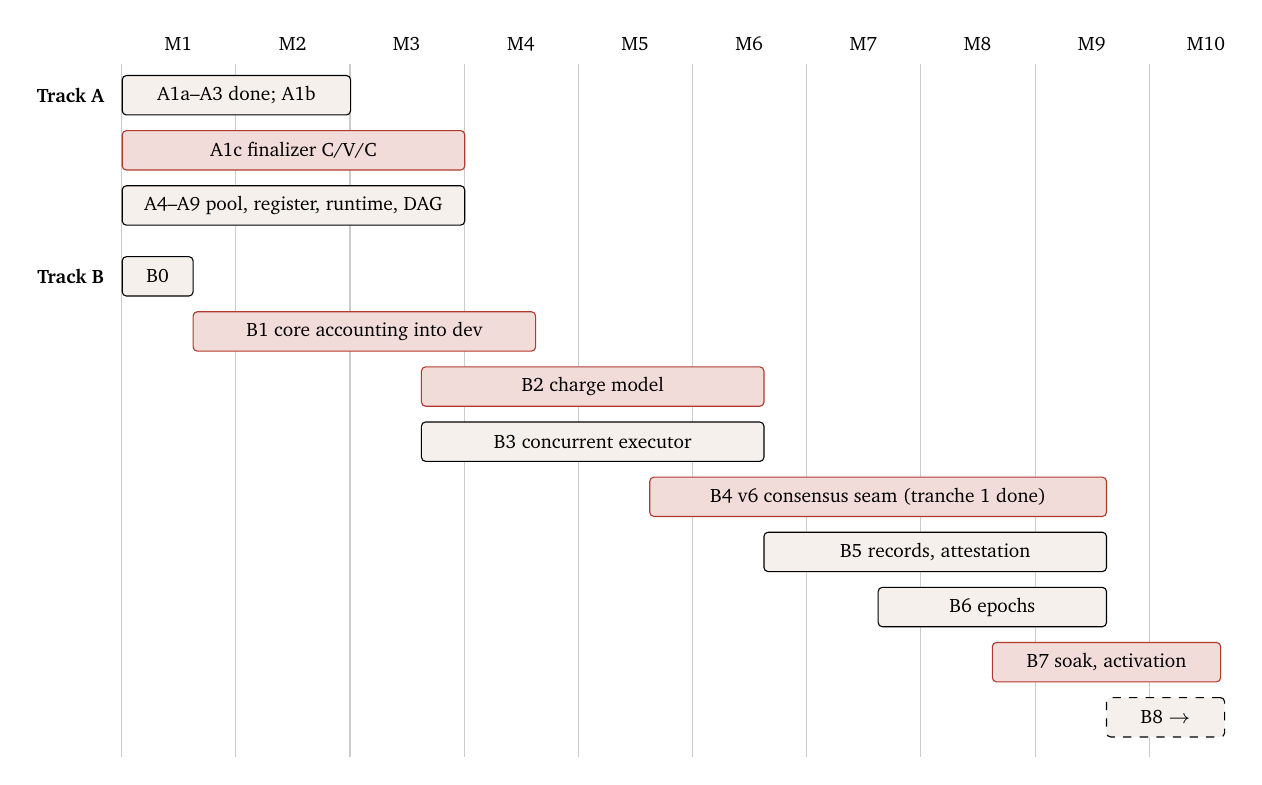
\begin{tikzpicture}[
  bar/.style={draw,rounded corners=1.5pt,fill=soft,font=\scriptsize,minimum height=0.5cm,anchor=west,inner sep=2pt},
  crit/.style={bar,fill=accent!18,draw=accent}]
\foreach \m in {0,...,9} { \draw[gray!40] (\m*1.45+1.7,0.4) -- (\m*1.45+1.7,-8.4); \node[font=\scriptsize] at (\m*1.45+2.42,0.65) {M\the\numexpr\m+1\relax}; }
\node[font=\scriptsize\bfseries,anchor=east] at (1.6,0) {Track A};
\node[bar,minimum width=2.9cm] at (1.7,-0.0) {A1a--A3 done; A1b};
\node[crit,minimum width=4.35cm] at (1.7,-0.7) {A1c finalizer C/V/C};
\node[bar,minimum width=4.35cm] at (1.7,-1.4) {A4--A9 pool, register, runtime, DAG};
\node[font=\scriptsize\bfseries,anchor=east] at (1.6,-2.3) {Track B};
\node[bar,minimum width=0.9cm] at (1.7,-2.3) {B0};
\node[crit,minimum width=4.35cm] at (2.6,-3.0) {B1 core accounting into dev};
\node[crit,minimum width=4.35cm] at (5.5,-3.7) {B2 charge model};
\node[bar,minimum width=4.35cm] at (5.5,-4.4) {B3 concurrent executor};
\node[crit,minimum width=5.8cm] at (8.4,-5.1) {B4 v6 consensus seam (tranche 1 done)};
\node[bar,minimum width=4.35cm] at (9.85,-5.8) {B5 records, attestation};
\node[bar,minimum width=2.9cm] at (11.3,-6.5) {B6 epochs};
\node[crit,minimum width=2.9cm] at (12.75,-7.2) {B7 soak, activation};
\node[bar,minimum width=1.5cm,dashed] at (14.2,-7.9) {B8 $\rightarrow$};
\end{tikzpicture}
\caption{Indicative sequencing in months, assuming three to four engineers on Track~B and the Casper team on Track~A. Shaded bars are on the critical path. Estimates, not commitments.}
\end{figure}

B2 and B3 can run in parallel once B1's core is in \code{dev}. B4 depends on B3's library interface and on A1--A3, because a v6 shard without the finality fixes would reproduce the consensus half of the loop. A1c is on the critical path: B7 activation needs it. Its precondition P4 should land early, because it checks A-LIN, which the v6 linearizer relies on. Tranche~1 of B4 ran ahead of B1--B3 by sharing one budget per block. The remaining B4 work picks up per-signature budgets when B1 lands. The overall estimate for B0--B7 is about ten calendar months with three to four engineers on Track~B. For comparison, the branch proposal estimates its order-then-execute phase alone at 4--9 engineer-months; this plan adds the core merge (B1), the charge model (B2) and the backpressure work.

\subsection{Ownership}

\begin{itemize}
\item \textbf{Casper team:} Track A, with the Casper Working Group owning A1c; the hook points of B4; B5 evidence classes; B6; answers to Q-1 to Q-7.
\item \textbf{Cost-accounting lane:} B1, B2, B3, and the \code{v6} module of B4.
\item \textbf{Formal methods:} the models and proofs listed with each exit criterion, and marking superseded scheduler-based models.
\item \textbf{File-I/O team:} coordination on the scheduler port in \code{dev} (decision~1).
\end{itemize}

%======================================================================
\section{Risks and open questions}

\subsection{Risks}

\begin{longtable}{@{}P{4.6cm}P{10.4cm}@{}}
\toprule
\textbf{Risk} & \textbf{Mitigation} \\
\midrule
\endhead
A-LIN fails (an LFB off a later LFB's main chain) & Linearizer checks and holds; the commit halts with \code{ALinViolation} (P4); Casper team confirms A-LIN from the clique oracle's spine argument, or documents the halt as the canonical response (Q-1). \\
A deadline cancels a commit part of the way through (\code{dev} today) & A1b times only the derivation; A1c makes the commit one atomic transaction. \\
Snapshot churn under load leaves no stable window & Freeze to the last stable snapshot, by default when the invalidation rate is high; Validate keeps the result safe; the invalidation metric is part of the soak gate. \\
Atomic commit changes the storage schema and the event wire format & New marker store and LFB pointer, included in soak snapshots; \code{BlockFinalisedV2} as a new enum variant; startup reconciliation; consumers already deduplicate or forward \code{commit_epoch}. \\
Host-work nondeterminism across hosts (bugs 10814, 10812) & Close in B2; cross-host replay in B3's exit criteria. \\
Finality remains the bottleneck after execution leaves consensus & A1--A3 are prerequisites for B4; pacing and lag gates in the design. \\
Core accounting cannot be separated from Casper plumbing & First task of B1; minimal plumbing behind \code{is_v6_shard()} if needed. \\
\code{dev} keeps moving (470 commits since the merge base) & Rebase B1 weekly; land in small PRs. \\
Scheduler port on \code{dev}'s file-I/O line conflicts with decision~1 & Agree with the file-I/O team before B1 lands. \\
Record size and retention & Per-block record cap; retention policy (Q-7); state sync from attested roots (Q-5). \\
Footprint marking incomplete for some interaction & Property test in \S\ref{sec:footprint} before R1 ships; R1 is not on the critical path. \\
Client changes & Clients size phlo limits to the linear estimate; Embers and the gateway need updates before activation. \\
\bottomrule
\end{longtable}

\subsection{Open questions for the Casper team}

\begin{longtable}{@{}P{1.0cm}P{14.0cm}@{}}
\toprule
\textbf{ID} & \textbf{Question} \\
\midrule
\endhead
Q-1 & Does every LFB lie on the main chain of every later LFB (A-LIN)? \emph{Measured October 16, 2026: not on legacy multi-parent shards.} The A1c integration run logged four commits whose candidate contains the previous LFB only through a secondary parent. P4 is therefore an alarm on legacy shards and a halt on v6 shards, where the state lineage is the main chain. \\
Q-2 & Which evidence class and penalty apply to misattestation, invalid records and inclusion-rule violations? \\
Q-3 & How many epochs of lag separate the attested bond state from the epoch that uses it? \\
Q-4 & May fork choice and the clique oracle give an equivocator zero weight as soon as the view holds the equivocation? \\
Q-5 & How much attesting stake makes a root acceptable for state sync? \\
Q-6 & How long may a node hold a block whose \code{bonds} field it cannot yet check? \\
Q-7 & Runner fallback distance $k$, per-block record cap, and record retention. \\
Q-8 & Threshold values: floor distance for pacing, executed-root lag for the envelope gate, pool admission cap. A3 sets defaults of 128 blocks and $64\times$ the per-block deploy limit. \\
Q-9 & Should the finalizer cursor survive a restart? The response proposes memory only for a first version. \\
Q-10 & May \code{propagate_ft_to_finalized_blocks} stay outside the atomic commit? It raises a monotone lower bound, so a partial crash heals itself. \\
Q-11 & Is \code{commit_epoch} counted per LFB or per boot? The response recommends per LFB. \\
Q-12 & Where do the asynchronous finalization effects run once \code{commit_lfb} is atomic? This design proposes after the commit, keyed to the marker, and idempotent. \\
\bottomrule
\end{longtable}

%======================================================================
\appendix
\section{Detailed stall findings}

The table lists the findings of the stall review beyond those in Section~\ref{sec:analysis}, by subsystem, with the lines at which each was located on \code{master} at \code{7264c98}. Severity is the review's estimate of the contribution to a stall that worsens under load.

\begin{longtable}{@{}P{2.3cm}P{7.9cm}P{3.6cm}P{1.0cm}@{}}
\toprule
\textbf{Subsystem} & \textbf{Finding} & \textbf{Location} & \textbf{Sev.} \\
\midrule
\endhead
Proposer & Unfinalized cone walked once per parent with full block decodes. & \code{block_creator.rs:1497-1725, 2085-2131} & High \\
Proposer & Whole pool sorted and encoded per selection, three times. & \code{block_creator.rs:269-279, 349-415} & Med \\
Proposer & Per-deploy WARN logged for every in-scope deploy on every proposal. & \code{block_creator.rs:1380-1440} & Med \\
Merge & Retry loop rebuilds branches and conflict map each pass. & \code{dag_merger.rs:705-752} & High \\
Merge & Stale-diff expansion runs one DAG search per block pair. & \code{dag_merger.rs:1855-1915} & Med \\
Merge & Dependency ordering cubic in branch size; \code{depends} allocates sets per call. & \code{dag_merger.rs:82-120, 1456-1502} & Med \\
Merge & \code{ChannelChange::combine} quadratic on hot channels. & \code{channel_change.rs:17-55} & Med \\
Merge & Block-index cache returns deep clones; bypasses its FIFO bound. & \code{interpreter_util.rs:1316-1342} & Med \\
Finality & Uncached LMDB metadata lookups inside \code{block_in_place}. & \code{block_dag_key_value_storage.rs:144-151} & High \\
Finality & FT propagation rescans up to 50{,}000 blocks under both write locks. & \code{block_dag_key_value_storage.rs:1699-1727} & Med \\
Finality & Estimator scoring walks $O(V \times (\text{tip}-\text{LCA}))$. & \code{estimator.rs:232-378} & Med \\
Finality & Redundant fault-tolerance oracle run after each LFB advance. & \code{finalization_runner.rs:571-576} & Med \\
Block processing & DAG membership via full representation per gossip message. & \code{block_admission.rs:34-67} & High \\
Block processing & Pendant full scan every 32 blocks with block decodes. & \code{buffer_resolver.rs:59-109} & Med \\
Block processing & Retriever sends serially, one hash at a time. & \code{block_retriever.rs:1032-1139} & Med \\
Block processing & Full snapshot computed per incoming block; cache keyed on DAG generation. & \code{block_processor.rs:548-553} & Med \\
RSpace & \code{put_continuation} formats a \code{Debug} string per waiting continuation. & \code{hot_store.rs:528-559, 1000} & Med \\
RSpace & Checkpoint CPU and LMDB writes on tokio workers. & \code{ispace_impl.rs:41-78} & Med \\
RSpace & History caches cleared in bulk; radix cache evicts arbitrary nodes. & \code{hot_store.rs:1091-1117}, \code{radix_tree.rs:875-890} & Med \\
Node & gRPC \code{find_deploy} server-side retry loop. & \code{deploy_grpc_service_v1.rs:570-643} & Med \\
Node & HTTP offload without an admission limit. & \code{shared_handlers.rs:626-640} & Low \\
\bottomrule
\end{longtable}

\section{Sources}

\begin{itemize}
\item \code{F1R3FLY-io/f1r3node-rust}, branches \code{master}, \code{dev} and \code{feature/cost-accounted-rho} at the commits listed on the first page.
\item \code{docs/casper/theory/cost-accounting-consensus-proposal.md} on \code{feature/cost-accounted-rho} (amended October 13, 2026): Greg Meredith's four expectations, the paper quotations, the decision records DR-64 to DR-124, the soak and profile data, and the proposal's \S7.
\item The cost-accounting papers in the F1R3FLY publications repository, as quoted in that proposal. This document did not read the papers directly; quotations are as the proposal gives them.
\item \code{docs/soak-benchmarks.md} on \code{master}, for the soak lifecycle and gates.
\item F1R3node Casper Working Group, ``A Live-and-Safe Finalizer-Progress Design: Response to Stall-Loop-Design \S5.10.1'', October 16, 2026, \code{F1R3FLY-io/publications}, \code{cost-accounting/stall-loop-design-5-10-1-response.tex}.
\item Branches \code{fix/finality-stall-track-a} and \code{feature/cost-accounted-ote} on \code{F1R3FLY-io/f1r3node-rust}, as pushed on October 16, 2026.
\end{itemize}

\end{document}
